\chapter{Introduction}
\label{intro}
\graphicspath{{Introduction/Images/}}

Asteroids are small rocky bodies in our solar system that are orbiting the Sun. These small bodies are basically the remnants from the process that formed the inner planets in our Solar System \cite{whyAsteroidsWeb}. Asteroids are mainly found in an orbit between Jupiter and Mars and as such are classified as \gls{MBO}. These \gls{MBO} range in size from a few meters to hundreds of kilometers, the largest one being 1 Ceres with a diameter of 948 km. A subset of the \gls{MBO}, called the \gls{NEA}, are asteroids whose orbits come extremely close to, and sometimes even cross, the orbit of the Earth \cite{jpl_asteroid_web}. Other small bodies in our small system, classified as asteroids when broadly speaking, are the Trojans (small bodies captured at Jupiter's Lagrange points 4 and 5), the \gls{TNO} (small bodies whose orbits around the Sun go beyond Neptune), the Centaurs (small bodies whose orbits lie in between Jupiter and Neptune) \cite{jpl_asteroid_web}. The asteroids in the main-belt tend to be more rocky in nature, however the small bodies beyond Jupiter tend to have a more icy-composition due to their relatively larger distance from the Sun \cite{jpl_asteroid_web}. A histogram plot depicting the distribution of \gls{MBO} is shown in \Cref{fig:mbo_distribution}. The gaps in the plot depict resonance in mean-motion between Jupiter and an asteroid \cite{jpl_asteroid_web}.
%
\begin{figure}[htb]
\centering
\captionsetup{justification=centering}
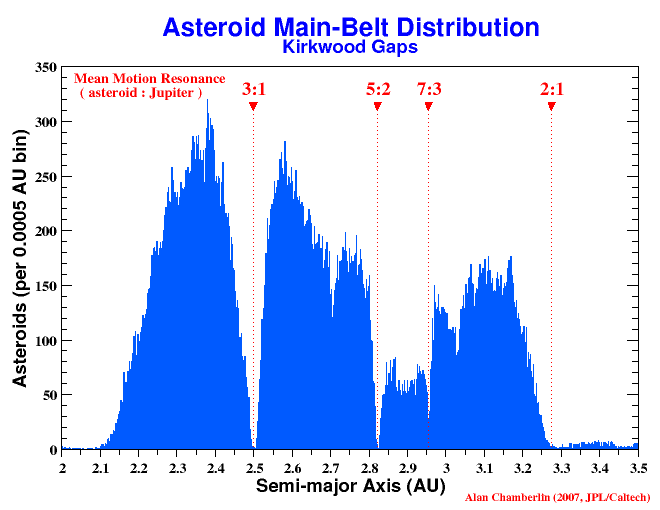
\includegraphics[width=\textwidth]{ast_histo-inverted.png}
\caption{Histogram plot depicting distribution of semi-major axis of 156,929 main-belt asteroids, created in June 2007 \cite{jpl_asteroid_web}.}
\label{fig:mbo_distribution}
\end{figure}
%

Asteroids don't only exist as single bodies in the Solar System, but they are also found in local multi-body systems consisting of two to even three asteroids. With advanced asteroid detection methods, astrophysicists have found over 190 multiple asteroid systems in the Solar System \cite{multipleAsteroids}. Contrary to intuition, these multiple asteroid systems exhibit a wide diversity in terms of the size ratios of the components, their mutual orbits and separation, implicating that the individual components evolved differently over time \cite{multipleAsteroids}. If a multi-asteroid system consists of two or three components, which are bound gravitationally, then it is termed as \textit{binary asteroids} or \textit{triple asteroids} respectively. Triple asteroids are also sometimes termed as \textit{trinary} or \textit{ternary} \cite{multipleAsteroidsTerminology}. Asteroid components that are not gravitationally bound but are genetically related, are termed as \textit{asteroid pairs}. Asteroid pairs where the larger asteroid is a binary or a triple asteroid, are termed as \textit{paired binaries} or \textit{paired triples}, respectively. The larger component in a binary or triple asteroid system or an asteroid pair, is referred to as the \textit{primary} and similarly the smaller component is referred to as the \textit{secondary} \cite{multipleAsteroidsTerminology}. Asteroids are further classified based on their dimensions and thermal properties, for which the reader should read the publication in \cite{multipleAsteroids}.

We now know what asteroids are and the different ways in which they are found in our Solar System, but is it important to study them? There are three major, and most commonly expressed, reasons to study asteroids in our solar system, and not just from a distance such as through radar telescopes placed on Earth, but also through in-situ exploration involving spacecrafts and surface probes. These reasons are mentioned as follows.
\begin{itemize}
\item Asteroids are basically the material left-over from formation of planets in our Solar System. Thus, they are the perfect source to study and understand the origins of the Solar System, as they have remained in the same pristine form since the birth of the Solar System, unlike the planets which have undergone massive topographical and atmospheric changes after their formation. The asteroids can provide valuable information on the chemical composition and initial conditions which led to the formation of planets, including Earth some 4.6 billion years ago. Several scientists have also hypothesized that water and life could have been brought about on Earth through an asteroid or comet and hence exploration of these small bodies could provide a definite answer to an age old question of how life began on Earth \cite{whyAsteroidsWeb}.
\item Asteroids have been hypothesized to have brought complex molecules to the surface of Earth that eventually resulted in life, but lately they have also been linked to the extinction of dinosaurs due to its impact with Earth. Earth is continuously bombarded with very small interplanetary material, most of which doesn't reach the surface of the Earth but gets evaporated in its atmosphere. However, every few 100 years, an asteroid spanning some tens of meter could impact Earth resulting in widespread damage, in the present case to life and property. But the impact from those will not cause the human race to extinct. But every 100,000 years or so, larger asteroids, spanning over tens of kilometer would impact the Earth, which will lead to extinction of life as we know it now. Although the probability of getting hit by an asteroid on such a large scale is low, it is still a statistical possibility and to be able to device strategies for active deflection of such asteroids, it is imperative that we understand more of the dynamics, properties and composition of the asteroids \cite{whyAsteroidsWeb}.
\item The third most important reason for us to study asteroids, is the fact that these small bodies are rich in raw materials or minerals. \gls{NEA} can be exploited for the resources that they possess and use it to build space structures or generate fuel for spacecrafts to enable human space exploration in farther reaches of the Solar System. By studying the asteroids, we can develop methods to tap the vast reservoirs of raw materials residing in them \cite{whyAsteroidsWeb}.
\end{itemize}

\section{Research problem}
In the previous section, we discussed what asteroids are and why its important to study them. In this section, we shall discuss, albeit broadly, the areas of research for the upcoming thesis work. The motivation for this literature study and the future thesis work arises from the fact that past in-situ space exploration activities have made use of explosive capsules to extract subsurface samples for analysis \cite{hayabusa2}. For asteroids with surface made of unconsolidated rock material or dust, use of explosive payloads to expose subsurface material could potentially result in the regolith being lofted from the surface of the asteroid. The lofted material could enter into a long term orbit, or a short term orbit concluding in re-impact of the lofted regolith back on the surface of the asteroid, or even escape the gravitational influence of the asteroid. This idea is fueled by a research paper \cite{idaEjectaErosion} which discusses the re-accretion and and escape of ejecta due to impact from impacts in the Ida system in the main-belt. The lofted regolith poses a serious threat to the safety of the spacecraft in orbit around the asteroid. To avoid any damage to it, it is necessary to develop models that can simulate the motion of the lofted regolith for a given asteroid, to as high an accuracy as possible, so that the mission design for asteroid exploration can account for it and ensure safety of the spacecraft. To do so we need to model the dynamics of the asteroid around the Sun, model the dynamical environment around the asteroid itself, and, although not limited to but also model the dynamics for multiple debris particles lofted from the asteroids surface and account for different perturbing forces that could affect the orbital motion of these particles. By running these simulation models we can compute trajectories for multiple particles at the same time and observe their long or short term behavior.

The tentative research questions shall be presented shortly. We say tentative because in the beginning, the report was aimed to focus on \textit{orbital motion of spacecraft around a binary asteroid system}. However, towards the period around which the report was being concluded, a thesis opportunity was offered from the \gls{CCAR} because of which the thesis topic was changed to \textit{orbital motion of regolith lofted from the surface of an asteroid}. The content of the report is nevertheless useful since it still discusses the dynamics around an asteroid with the difference that instead of a spacecraft, now it will be applied to lofted regolith material. Due to the sudden shift in the focus of the thesis at the time of writing this report, the research questions presented below should be considered as only tentative. The final research questions or problem statements will be mentioned in the final thesis report. The core questions are listed as follows:
\begin{itemize}
\item Simulate, observe and characterize the motion of regolith lofted from the surface of an asteroid for extended periods of time.
\item Does the lofted regolith enter a stable or unstable orbit? What are the corresponding initial conditions and can they be generalized for different asteroids?
\item What is the correlation, if any, between the size of the lofted material against stable or unstable orbital motion? Can a critical size for the lofted material be determined, for the asteroid under study, which would differentiate between stable and unstable orbital motion for the lofted material?
\item In case of stable orbits, are the orbits planar or spatial periodic?
\item In case of an unstable orbit, does the lofted regolith fall back to the surface of the asteroid or does it escape the gravitational influence of the asteroid? Can this behavior be also generalized for a different asteroid?
\item What is the subsequent motion of the regolith that re-impacts on the surface of the asteroid?
\item For a regolith sample return mission based on a touch-and-go technique (such as the \gls{OSIRIS-REx} mission), is it possible to retrieve a sample without causing adjacent surface material to be lofted in to an orbit around the asteroid?
\item For a subsurface sample return mission involving surface detonation (such as the Hayabusa-2 mission), how can the dangers of spacecraft damage from lofted regolith be averted or avoided?
\end{itemize}

\section{Outline of the report}
This literature study report tackles the problem of modeling particle dynamics and solving it in a systematic way. We begin by first describing the various missions that have been to asteroids in the past or are being operated currently along with missions planned for the future in \Cref{heritage}. \Cref{gravpot} discusses the various gravitational potential models that exist and have been applied in past for theoretical studies on orbital mechanics of or around asteroids along with the advantages and disadvantages of each model. \Cref{perturb} presents the relevant orbit perturbation models for working with particle dynamics around asteroids. \Cref{F2BP} begins with a brief introduction to relatively low-fidelity full two-body problem models that have been extensively applied in the past following which an extensive discussion on mutual potential and coupled equations of motion for binary polyhedron-based asteroids is presented. \Cref{RF3BP} begins by introducing the relatively low-fidelity restricted three-body problem but the chapter focuses more on the dynamics of a particle around binary asteroid modeled as two polyhedrons. A linearization technique to reduce simulation loads has also been introduced in that chapter. \Cref{integ} describes and compares the various numerical integration methods; an integrator is needed to propagate the orbital motion of a particle around an asteroid. \Cref{MCS} briefly describes the Monte Carlo simulation technique which will be utilized in our simulation package to generate multiple debris particles at the surface of an asteroid. \Cref{DST} presents some basic concepts on dynamical systems theory such as poincar\'e maps which are used when one wants to characterize the motion of an orbiting particle. And finally, \Cref{conclusion} concludes the literature study report.
